% Does a tyre-degradation model transfer?
%
% Compile on Overleaf (pdfLaTeX). numbers.tex is GENERATED by
% scripts/make_paper_numbers.py -- this file contains no digits of its own,
% which is deliberate: see the header of that script.
\documentclass[11pt,a4paper]{article}

\usepackage[utf8]{inputenc}
\usepackage[T1]{fontenc}
\usepackage[margin=1in]{geometry}
\usepackage{amsmath,amssymb}
\usepackage{booktabs}
\usepackage{graphicx}
\usepackage{caption}
\usepackage[hidelinks]{hyperref}
\usepackage{natbib}
\usepackage{microtype}

% GENERATED by scripts/make_paper_numbers.py -- do not edit by hand.
%
% Every number in main.tex is one of these macros. The manuscript
% contains no digits of its own, so it cannot drift from the data the
% way this project's prose repeatedly has -- regenerate the artifacts,
% regenerate this file, and the paper is correct or CI fails.

\newcommand{\NDecisions}{1,280}
\newcommand{\NDecisionsFone}{357}
\newcommand{\NRaceSeasons}{205}
\newcommand{\NCircuitClasses}{51}
\newcommand{\NClasses}{7}
\newcommand{\NCircuitsFone}{25}
\newcommand{\NCoefficientsFone}{73}
\newcommand{\NRacesFone}{104}
\newcommand{\SeasonsFone}{2022--2026}
\newcommand{\NDecisionsFoneScope}{357}
\newcommand{\NRacesElms}{42}
\newcommand{\SeasonsElms}{2021--2025}
\newcommand{\NClassesElms}{2}
\newcommand{\NCircuitsElms}{9}
\newcommand{\NDecisionsElms}{171}
\newcommand{\NRacesImsa}{136}
\newcommand{\SeasonsImsa}{2021--2026}
\newcommand{\NClassesImsa}{3}
\newcommand{\NCircuitsImsa}{13}
\newcommand{\NDecisionsImsa}{632}
\newcommand{\NRacesWec}{27}
\newcommand{\SeasonsWec}{2022--2026}
\newcommand{\NClassesWec}{1}
\newcommand{\NCircuitsWec}{11}
\newcommand{\NDecisionsWec}{120}
\newcommand{\NFinishers}{5}
\newcommand{\NCars}{5}
\newcommand{\LookbackFone}{5}
\newcommand{\LookbackEnd}{3}
\newcommand{\MinFirstStopFone}{8}
\newcommand{\MinFirstStopEnd}{6}
\newcommand{\NRivals}{2}
\newcommand{\NDraws}{5,000}
\newcommand{\MinFinalStint}{3}
\newcommand{\NCoefCrossingZero}{16}
\newcommand{\PctCoefCrossingZero}{22}
\newcommand{\PctCompoundOverlap}{75}
\newcommand{\BestTransfer}{+0.573}
\newcommand{\BestTransferWhere}{Lime Rock GTD}
\newcommand{\TransferThreshold}{0.2}
\newcommand{\NTransferAboveTwo}{5}
\newcommand{\GTThreeMean}{+0.104}
\newcommand{\GTThreeCI}{[+0.050, +0.170]}
\newcommand{\ProtoMean}{-0.060}
\newcommand{\ProtoCI}{[-0.199, +0.021]}
\newcommand{\TransferDiff}{+0.164}
\newcommand{\TransferDiffCI}{[+0.059, +0.312]}
\newcommand{\TransferP}{0.0009}
\newcommand{\BestTransferFolds}{3}
\newcommand{\BestTransferSpread}{0.024}
\newcommand{\ThinTransfer}{+0.497}
\newcommand{\ThinTransferWhere}{Lime Rock GTD PRO}
\newcommand{\ThinTransferFolds}{2}
\newcommand{\ThinTransferLow}{+0.357}
\newcommand{\ThinTransferHigh}{+0.638}
\newcommand{\ThinTransferSpread}{0.281}
\newcommand{\PitLossR}{-0.982}
\newcommand{\PitLossRCI}{[-0.986, -0.745]}
\newcommand{\CheapStopEdge}{22.5}
\newcommand{\NAboveEdge}{150}
\newcommand{\NTyreLimitedAboveEdge}{0}
\newcommand{\NTyreLimited}{25}
\newcommand{\EdgeWithoutDefining}{13.2}
\newcommand{\EdgeDropPct}{41}
\newcommand{\FoneMedian}{+10}
\newcommand{\FoneLateShare}{80}
\newcommand{\FoneLateMedian}{12}
\newcommand{\ElmsMedian}{+2}
\newcommand{\ElmsLateShare}{56}
\newcommand{\ElmsCautionShare}{20}
\newcommand{\ImsaMedian}{+12}
\newcommand{\ImsaLateShare}{83}
\newcommand{\ImsaCautionShare}{53}
\newcommand{\WecMedian}{+1}
\newcommand{\WecLateShare}{30}
\newcommand{\WecCautionShare}{8}
\newcommand{\NScored}{1,263}
\newcommand{\ElmsLmptwoModelError}{2}
\newcommand{\ElmsLmptwoBoneError}{3}
\newcommand{\ElmsLmptwoBtwoError}{45}
\newcommand{\ElmsLmptwoBthreeError}{4}
\newcommand{\ElmsLmptwoProAmModelError}{3}
\newcommand{\ElmsLmptwoProAmBoneError}{2}
\newcommand{\ElmsLmptwoProAmBtwoError}{45}
\newcommand{\ElmsLmptwoProAmBthreeError}{4}
\newcommand{\FoneModelError}{10}
\newcommand{\FoneBoneError}{11}
\newcommand{\FoneBtwoError}{7}
\newcommand{\FoneBthreeError}{--}
\newcommand{\ImsaGtdModelError}{12}
\newcommand{\ImsaGtdBoneError}{7}
\newcommand{\ImsaGtdBtwoError}{18}
\newcommand{\ImsaGtdBthreeError}{14}
\newcommand{\ImsaGtdproModelError}{12}
\newcommand{\ImsaGtdproBoneError}{9}
\newcommand{\ImsaGtdproBtwoError}{33}
\newcommand{\ImsaGtdproBthreeError}{15}
\newcommand{\ImsaGtpModelError}{9}
\newcommand{\ImsaGtpBoneError}{9}
\newcommand{\ImsaGtpBtwoError}{54}
\newcommand{\ImsaGtpBthreeError}{14}
\newcommand{\WecHypercarModelError}{2}
\newcommand{\WecHypercarBoneError}{2}
\newcommand{\WecHypercarBtwoError}{39}
\newcommand{\WecHypercarBthreeError}{1}
\newcommand{\NClassesRuleWins}{5}
\newcommand{\NClassesBoneWins}{3}
\newcommand{\NClassesRuleTies}{1}
\newcommand{\NClassesOptimiserWins}{1}
\newcommand{\NClassesScored}{7}
\newcommand{\ElmsLmptwoPitLoss}{62}
\newcommand{\ElmsLmptwoProAmPitLoss}{64}
\newcommand{\ImsaGtdPitLoss}{24}
\newcommand{\ImsaGtdproPitLoss}{40}
\newcommand{\ImsaGtpPitLoss}{57}
\newcommand{\WecHypercarPitLoss}{74}
\newcommand{\TrackPositionRange}{14}
\newcommand{\NCircuitsSwap}{25}
\newcommand{\SwapLowestCircuit}{Monaco}
\newcommand{\SwapHighestCircuit}{Las Vegas}
\newcommand{\SwapLowest}{0.0047}
\newcommand{\SwapLowestSd}{0.0016}
\newcommand{\SwapLowestRaces}{4}
\newcommand{\SwapHighestRaces}{3}
\newcommand{\SwapRunnerUpRatio}{4.1}
\newcommand{\SwapBetweenSd}{0.0104}
\newcommand{\SwapWithinSd}{0.0103}
\newcommand{\UndercutClosedMedian}{-1}
\newcommand{\UndercutShareImproving}{19}
\newcommand{\UndercutSpearman}{-0.15}
\newcommand{\SwapLowestClosedMedian}{+0.5}
\newcommand{\SwapLowestDecisions}{8}
\newcommand{\NIdentifiability}{0.691}


\title{Does a tyre-degradation model transfer?\\
\large Cross-championship evidence and a retrospective audit of
\NDecisions{} real pit-stop decisions}

\author{Mohammed Reda Medjadj\thanks{Independent.
Code, data and every figure in this paper:
\url{https://github.com/mohammedmedjadj/Motorsport-Strategy-Lab}.
Archived and citable at
\url{https://doi.org/10.5281/zenodo.22726130}.}}

\date{\today}

\begin{document}
\maketitle

\begin{abstract}
Race-strategy models are typically fitted and validated within one
championship, often within one race. Two questions that follow are rarely
asked: does a fitted model predict a season it has never seen, and does its
recommendation resemble what a professional team actually did? We answer both
on \NClasses{} car classes across four championships --- Formula~1, WEC, IMSA
and ELMS --- using one protocol applied identically to all of them.

Three results. First, tyre-degradation slopes transfer as a property of the
\emph{circuit-class}, not of the championship: of \NCircuitClasses{}
circuit-classes measured by leave-one-race-out, only \NTransferAboveTwo{} reach
a within-stint $R^2$ of $\TransferThreshold{}$, with a maximum of \BestTransfer{} at
\BestTransferWhere{}. GT3 classes transfer measurably better than prototype
classes (difference \TransferDiff{}, 95\% CI \TransferDiffCI{}, permutation
$p = \TransferP{}$), but a near-specification control field fails exactly as the
Balance-of-Performance-adjusted fields do, ruling out heterogeneous machinery as
the cause. Second, whether an extra stop can ever pay is set by the cost of the
stop rather than by the car: across \NRaceSeasons{} race-seasons the class-level
correlation between median pit loss and the share of tyre-limited races is
$\PitLossR{}$ (95\% CI \PitLossRCI{}), and \NAboveEdge{} race-seasons above a
\CheapStopEdge{}\,s pit loss contain \NTyreLimitedAboveEdge{} tyre-limited race.
Third, replaying \NDecisions{} real first pit stops through an exact optimiser
shows it stopping later than teams did on \FoneLateShare{}\% of Formula~1
decisions, by a median of \FoneLateMedian{} laps. Both explanations we proposed
for this were tested and both failed, and three rule-of-thumb baselines scored
on the same decisions beat it in \NClassesRuleWins{} of
\NClassesScored{} classes.

We report the third result as measured and unexplained. Two estimators built for
this work were validated on synthetic data and then withdrawn when they failed
on real fields, and both withdrawals are written up here.
\end{abstract}

\section{Introduction}

A pit stop is a decision under uncertainty with a measurable cost. The
literature on optimising it is small but real, and this paper's contribution is
not another optimiser. It is a pair of validation questions that the existing
work, for understandable reasons, does not ask.

The first is \emph{transfer}. A degradation model is fitted on races that have
happened and used on a race that has not. Whether a slope fitted on past seasons
of a circuit predicts the next season of that circuit is an empirical question,
and answering it requires holding a season out --- which in turn requires more
than one season, and ideally more than one championship.

The second is \emph{agreement with practice}. A model that recommends a stop lap
can be compared to the lap a team actually chose. This is not a claim about
which was faster; it is a measurement of where a model and a professional pit
wall part company, and by how much.

Both questions need breadth to answer, and breadth is what this work supplies:
one protocol, four championships, \NClasses{} car classes, every quantity
measured from published timing or absent.

\section{Related work}

Race-strategy research is largely about building the optimiser. The methods vary
widely --- discrete-event simulation, Monte Carlo, dynamic programming,
mixed-integer programming, reinforcement learning, game theory --- and the goal
is consistent: compute a better plan than a team would otherwise choose.

\citet{bekker2009} give the earliest sustained operations-research treatment,
simulating a full race with overtaking and traffic under the refuelling rules of
the time. \citet{heilmeier2018} introduce the lap-time decomposition that much of
the later work rests on, combining fuel mass, tyre degradation and driver
effects, and \citet{heilmeier2020mc} extend it to a probabilistic simulation
sampling accidents, safety cars and lap-time variability. \citet{heilmeier2020nn}
then train neural networks on that simulation's output to make calls in real
time. \citet{carrasco2022} give an exact dynamic program over stop laps and
compound choice, extended to a stochastic version, and \citet{aguad2024}
formulate the problem as a zero-sum feedback Stackelberg game between two
drivers, finding that a strategic competitor gains over 15\% in winning odds.
Outside Formula~1, \citet{vankampen2022} solve endurance stint planning and
powertrain operation jointly for an electric car under thermal limits. Recent
work adds learning: \citet{thomas2025} apply explainable reinforcement learning
to compound and stop timing, \citet{fieni2025} combine a mixed-integer program
with an RL agent over energy, tyre wear and pit timing, and \citet{todd2025}
forecast tyre energy from team-internal telemetry. \citet{santillana2026}
deploys a calibrated real-time Monte Carlo engine live, generating
natural-language briefings faithful to its own probabilistic state.

Two things are rare across all of it, and together they define what this paper
adds.

The first is out-of-sample validation of the fitted parameters. A tyre model is
fitted and its quality reported on the data it was fitted to. \citet{cappello2025}
come closest, building a Bayesian state-space model of degradation from the same
public timing source used here, with lap time as fuel mass plus a latent tyre
state and pit stops as resets. Their evaluation is one race, and they state
explicitly that generalising across races or circuits is future work for which
they offer no empirical evidence. They also report compound-specific degradation
differences as not statistically distinct --- an observation consistent with the
instability we measure at scale.

The second is comparison against what teams actually did. Optimisers get
compared to other optimisers, to author-constructed baselines, or to the optimum
under the model's own assumptions. \citet{bekker2009} compare to real races, and
\citet{aguad2024} compare strategic against non-strategic agents inside their
own game, but we are not aware of work that replays a large sample of real
pit-stop decisions and reports where the optimiser and the pit wall diverge.

We should be clear about how narrow the contribution is. The modelling here is
not more sophisticated than \citet{heilmeier2020mc} or \citet{aguad2024}; in
places it is deliberately simpler, and it ignores energy management entirely.
What is different is that one protocol is applied across four championships,
that the resulting parameters are tested on seasons they were not fitted to, and
that the optimiser is then confronted with \NDecisions{} real decisions. Two of
the three results that come back are negative.

\section{Data and protocol}

\subsection{Sources and scope}

Formula~1 lap timing, tyre compound and per-lap track status come from the
FastF1 API. WEC, IMSA and ELMS timing comes from a community-maintained
endurance dataset carrying lap times, stint structure and flag state but
\emph{not} tyre compound. The endurance degradation models are therefore
net-slope models where the Formula~1 one is per compound, and that asymmetry is
restated wherever the two are compared. Table~\ref{tab:scope} gives the scope.

\begin{table}[htbp]
\centering
\caption{Scope. A race-season is one class at one circuit in one season, which
is the unit everything here is fitted and reported on.}
\label{tab:scope}
\begin{tabular}{lrrrrl}
\toprule
& Classes & Circuits & Race-seasons & Replayed decisions & Seasons \\
\midrule
Formula~1 & 1 & \NCircuitsFone{} & \NRacesFone{} & \NDecisionsFone{} & \SeasonsFone{} \\
IMSA      & \NClassesImsa{} & \NCircuitsImsa{} & \NRacesImsa{} & \NDecisionsImsa{} & \SeasonsImsa{} \\
ELMS      & \NClassesElms{} & \NCircuitsElms{} & \NRacesElms{} & \NDecisionsElms{} & \SeasonsElms{} \\
WEC       & \NClassesWec{} & \NCircuitsWec{} & \NRacesWec{} & \NDecisionsWec{} & \SeasonsWec{} \\
\bottomrule
\end{tabular}
\end{table}

Nothing is imputed. Where a source lacks a quantity the affected layer is not
fitted, and the gap goes on the record as a gap.

\subsection{Degradation}

For driver--race $i$ and lap $\ell$ within stint $s$, with tyre age $a$ and
compound $c$,
%
\begin{equation}
y_{i\ell} \;=\; \alpha_i \;+\; \phi\,\ell \;+\; \sum_{k=1}^{d}\beta_{c,k}\,a_{i\ell}^{\,k} \;+\; \varepsilon_{i\ell},
\label{eq:degradation}
\end{equation}
%
where $y$ is lap time, $\alpha_i$ is a driver--race fixed effect absorbing car
pace, driver pace and track conditions, and $\phi\ell$ is a fuel-burn proxy that
is identified only where refuelling is prohibited. In endurance, where cars
refuel, $\ell$ is replaced by laps since the last refuelling stop and the
compound index drops out, leaving a single net slope $\beta_1$.

Equation~\ref{eq:degradation} is estimated by ordinary least squares through
a Moore--Penrose pseudoinverse,
which handles the rank-deficient cases --- a driver--race seen on one compound
only. The polynomial degree $d \in \{1,2\}$ is chosen per circuit by
leave-one-race-out cross-validation.

Standard errors are cluster-robust (CR1) on the driver--race and referred to
$t(G-1)$ rather than the normal \citep{cameron2015}. The clustering is not
decorative: lap-to-lap errors within one driver's race are strongly dependent,
and a coverage simulation on synthetic races with realistic between-unit slope
variation puts the classical 95\% interval at roughly 75\% coverage against 95\%
for the robust one.

\begin{figure}[htbp]
\centering
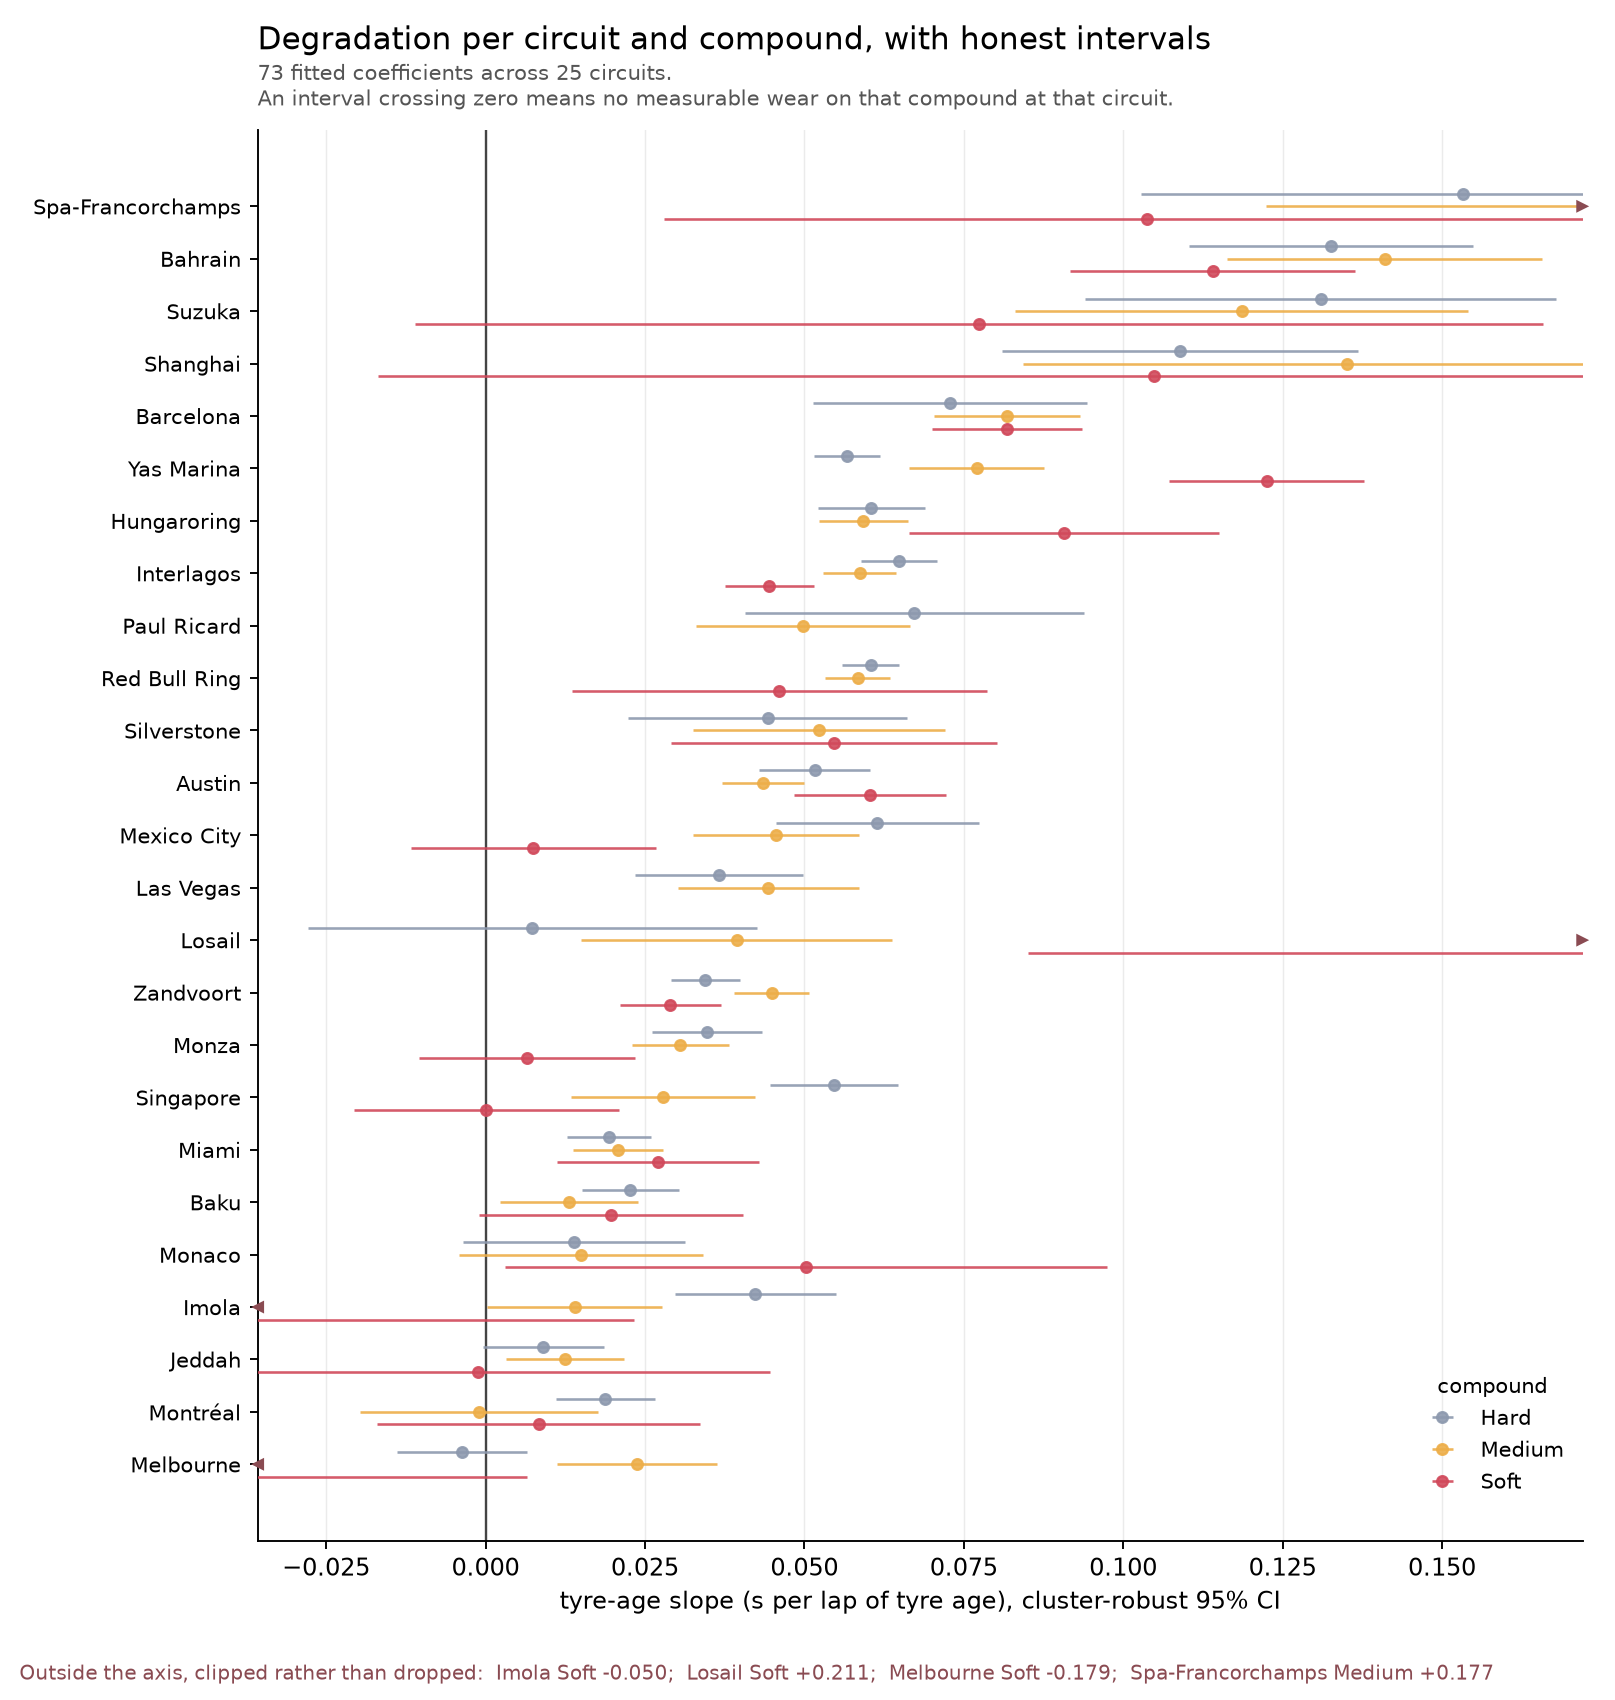
\includegraphics[width=0.82\textwidth]{../reports/figures/s3_f1_degradation.png}
\caption{The fitted object itself: linear tyre-degradation coefficients for
Formula~1, by circuit and compound, with cluster-robust intervals.
\NCoefficientsFone{} coefficients across \NCircuitsFone{} circuits. Points
outside the plotted range are clipped and then named under the axis, because a
handful of extremes otherwise compresses every other circuit into a tenth of
the width. Dropping them silently would be the same defect as any other
silent narrowing here.}
\label{fig:degradation}
\end{figure}

Figure~\ref{fig:degradation} is worth reading before the results, because two
features of it constrain everything after. \NCoefCrossingZero{} of the
\NCoefficientsFone{} fitted slopes, \PctCoefCrossingZero{}\%, have a
cluster-robust interval containing zero: on those circuit--compound pairs we
cannot distinguish tyre degradation from none. And within a circuit,
\PctCompoundOverlap{}\% of compound pairs have overlapping intervals, so the
compound distinction the Formula~1 model carries is largely unresolved by the
data behind it. Both are reported, and neither is screened out. A slope that
cannot
be distinguished from flat is still the measurement we have, and dropping the
ones that disappoint is how a transfer result gets manufactured.
Section~\ref{sec:threats} returns to what this costs.

\subsection{Transfer}

Fit on every season of a circuit-class but one, predict the held-out season, and
score the within-stint demeaned residual:
%
\begin{equation}
R^{2}_{\text{within}} \;=\; 1 - \frac{\sum_{s}\sum_{\ell \in s}\bigl(\tilde{y}_{\ell} - \tilde{\hat{y}}_{\ell}\bigr)^{2}}{\sum_{s}\sum_{\ell \in s}\tilde{y}_{\ell}^{\,2}},
\qquad
\tilde{x}_{\ell} = x_{\ell} - \overline{x}_{s}.
\label{eq:transfer}
\end{equation}
%
The demeaning in Equation~\ref{eq:transfer} is what makes this a test of the
\emph{shape} of
degradation rather than of pace. A driver--race intercept fitted on training
data cannot be observed on a held-out race, so comparing raw lap times would
leak information through $\alpha_i$.

\subsection{The multi-stop dynamic program}

For an endurance race of $L$ laps with green pace $p$, net slope $\beta$, pit
loss $\pi$ and fuel range $F$, a plan is a partition of $L$ into stints
$(n_1,\dots,n_{m+1})$ with $m$ stops. Total time under the fitted model is
%
\begin{equation}
T(n_1,\dots,n_{m+1}) \;=\; m\pi \;+\; \sum_{j}\left(n_j p + \beta\,\frac{n_j(n_j+1)}{2}\right),
\label{eq:dp}
\end{equation}
%
subject to $n_j \le F$ for every stint. The triangular sum is the accumulated
tyre loss over a stint of $n_j$ laps. We use it exactly, not as the
$\beta n_j^{2}/2$ integral --- they differ by $\beta n_j / 2$, which is about a
second over a forty-lap stint and is the only quantity the stop decision
compares against $\pi$.

Because $T$ in Equation~\ref{eq:dp} is separable across stints given $m$, the minimum over plans is a
one-dimensional dynamic program in remaining laps, solved exactly for each $m$
from the fuel minimum $\lceil L/F \rceil - 1$ upward. A race is called
\emph{tyre-limited} when the time-optimal $m$ exceeds that fuel minimum.

\subsection{The Monte Carlo engine and the decision audit}

The single-next-stop engine evaluates every candidate pit lap over
\NDraws{} shared realisations. Each draw resamples the degradation and fuel
coefficients from their cluster-robust posteriors ($t(G-1)$ scaled by the
estimated standard errors), the neutralisation hazard from its Gamma posterior,
and lap noise at the cross-validated residual scale. Candidates share the same
draws, so a comparison between two pit laps carries no unrelated sampling
noise. Plans leaving fewer than \MinFinalStint{} laps after the stop are
excluded.

The audit replays real decisions; it does not forecast them. For every race
with a fitted model, the top \NFinishers{} classified finishers in Formula~1
(\NCars{} cars in endurance) who made at least one stop are replayed at their
\emph{first} stop. The model is asked \LookbackFone{} laps before that stop in
Formula~1 and \LookbackEnd{} in endurance, given the state as it was, and its
recommended lap is compared to the team's. Stops earlier than lap
\MinFirstStopFone{} (\MinFirstStopEnd{} in endurance) are excluded as incidents
rather than strategy. Rivals keep their real, historically observed plans: the
decision under study is one car's, the rest of the world is as it happened.

This is what makes the comparison possible and also what stops it being a
prediction claim. The decision point is defined relative to a stop that already
happened.

\subsection{The three baselines}

Scored on the same decisions, from the same artifacts, on absolute lap error
against the team's stop.

\textbf{B1, fixed interval.} Divide the race into equal stints:
$\ell^{\star} = \operatorname{round}\!\left(kL/(m+1)\right)$ for the $k$th of
$m$ stops. Uses no fitted quantity at all.

\textbf{B2, threshold.} Stop on the first lap at which the stint's accumulated
tyre loss exceeds the pit loss,
%
\begin{equation}
\beta\,\frac{a(a+1)}{2} \;>\; \pi,
\qquad\text{firing at}\qquad
a^{\star} = \frac{-1 + \sqrt{1 + 8\pi/\beta}}{2}.
\label{eq:threshold}
\end{equation}
%
Equation~\ref{eq:threshold} uses the fitted slope and the measured pit loss,
and nothing else --- no fuel
term, no neutralisation hazard, no distribution over outcomes. The gap between
B2 and the full engine is precisely what the Monte Carlo buys.

\textbf{B3, fuel deadline.} Run the tank out. Undefined in Formula~1, where
refuelling has been prohibited since 2010, and reported as undefined rather than
substituted with the race end.

Where a rule cannot fire --- B2 on a tyre that never accumulates enough loss
before the flag --- no lap is returned and that decision is not scored for that
rule. Coverage is reported alongside every error, because a rule answering a
fifth of the decisions and landing close on those has not beaten one that
answers all of them.

\section{Result 1: transfer is a property of the circuit-class}
\label{sec:transfer}

\begin{figure}[htbp]
\centering
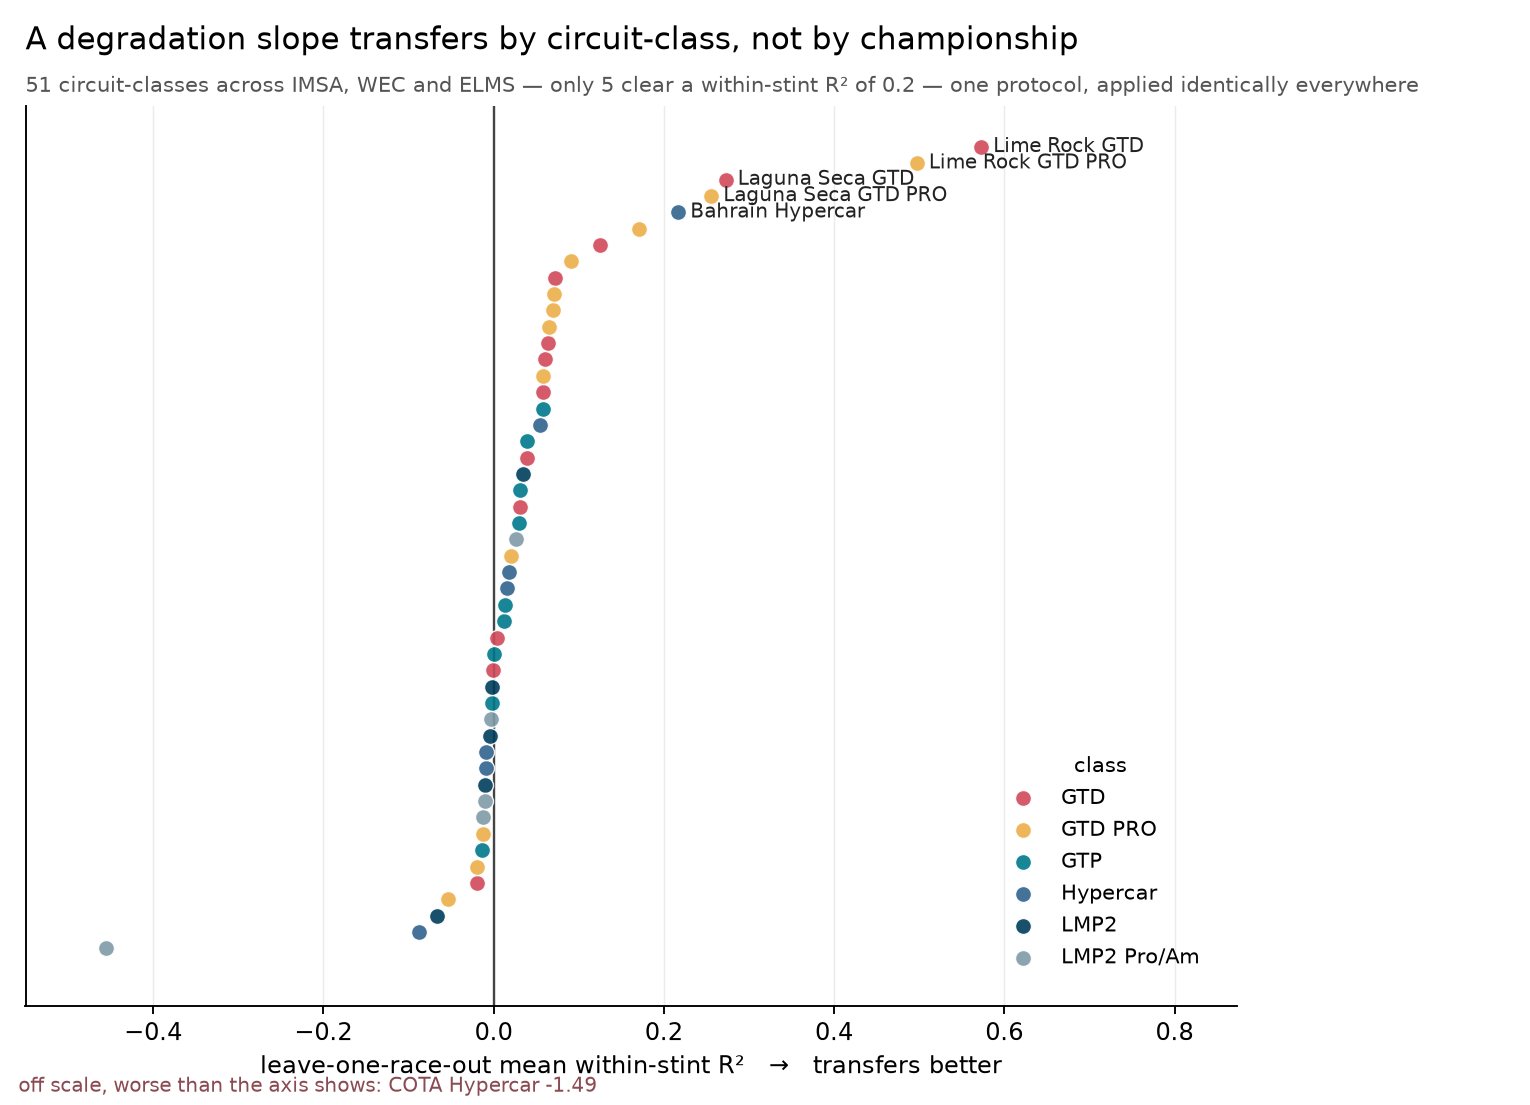
\includegraphics[width=0.86\textwidth]{../reports/figures/r1_transfer.png}
\caption{Leave-one-race-out mean within-stint $R^2$, one point per
circuit-class. Of \NCircuitClasses{} measured, \NTransferAboveTwo{} clear
$\TransferThreshold{}$.}
\label{fig:transfer}
\end{figure}

Figure~\ref{fig:transfer} shows the distribution. The maximum is
\BestTransfer{} at \BestTransferWhere{}; almost everywhere else a slope fitted
on past seasons predicts the next one no better than that season's own mean.

Grouping by car type, GT3 classes average \GTThreeMean{} (95\% CI \GTThreeCI{})
against \ProtoMean{} (\ProtoCI{}) for prototypes. The difference is
\TransferDiff{} with a 95\% cluster bootstrap interval of \TransferDiffCI{}, and
a permutation test on the group labels gives $p = \TransferP{}$. Both are
reported because they fail differently: the bootstrap assumes the clusters
resemble their population, the permutation assumes only exchangeability under
the null. Resampling is at the circuit-class, never the fold --- folds inside a
circuit-class share a pooled fitted slope, and treating them as independent
would roughly quadruple the apparent sample.

The obvious explanation for instability is heterogeneous, performance-balanced
machinery. We can rule it out. ELMS LMP2 is a near-specification class --- one
chassis, one engine, no Balance of Performance --- and its slopes fail to
transfer exactly as the balanced GT3 fields do. The instability is not the
hardware. Where transfer does occur it tracks short circuits with cheap
stops, which is the same axis Result~2 turns on.

\section{Result 2: the cost of the stop sets the strategy regime}

\begin{figure}[htbp]
\centering
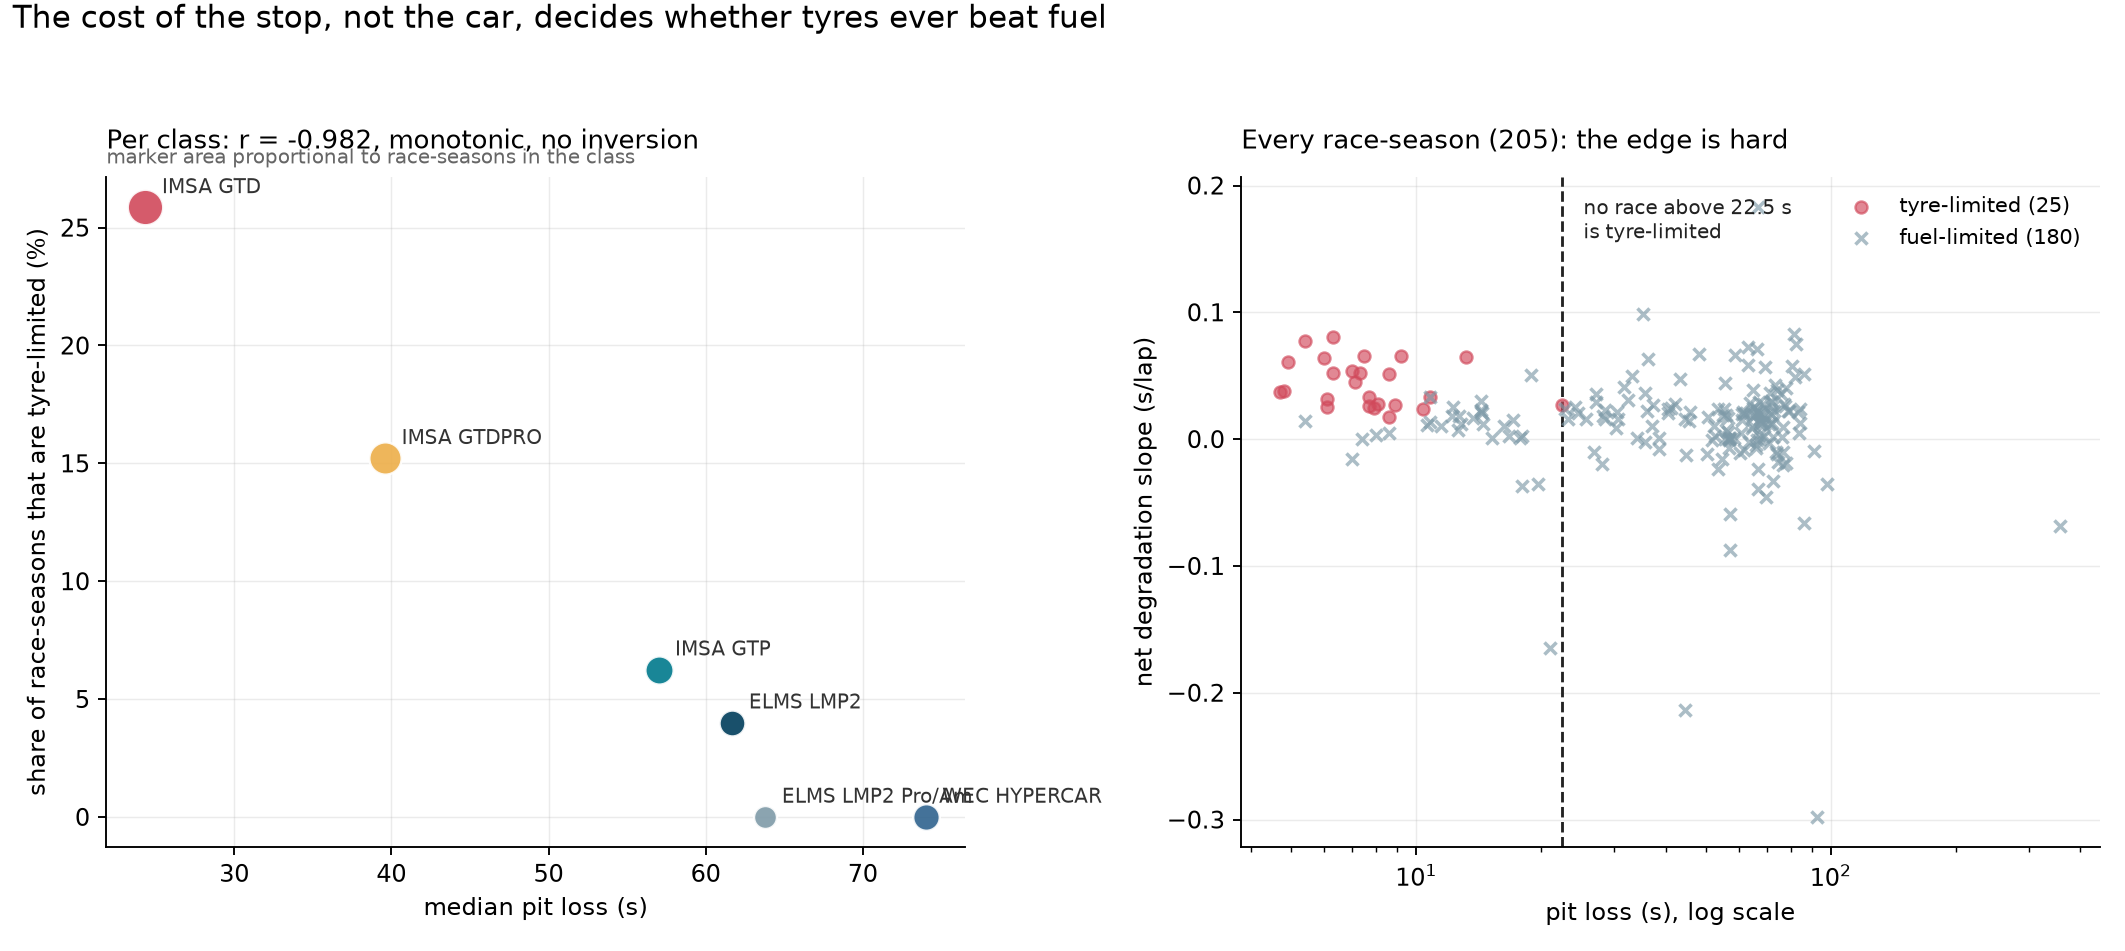
\includegraphics[width=\textwidth]{../reports/figures/r2_pit_loss_rule.png}
\caption{Left: class-level median pit loss against the share of race-seasons
where the tyre-optimal plan needs more stops than the fuel minimum. Right: every
race-season, with the empirical edge marked.}
\label{fig:pitloss}
\end{figure}

Figure~\ref{fig:pitloss} plots the rule. An exact dynamic program plans each
endurance race under a hard fuel constraint
and reports whether the tyre-optimal plan requires more stops than the fuel
minimum. Across \NRaceSeasons{} race-seasons, \NTyreLimited{} are tyre-limited.

The class-level correlation between median pit loss and tyre-limited share is
$\PitLossR{}$ with a 95\% interval of \PitLossRCI{}, monotonic across all
classes with no inversion. That interval is bootstrapped over \emph{races},
recomputing each class summary inside every replicate; bootstrapping the class
summaries themselves would give an interval over six fixed championships, which
is not a source of variation that exists.

At race level, \NAboveEdge{} of \NRaceSeasons{} race-seasons have a pit loss
above \CheapStopEdge{}\,s and \NTyreLimitedAboveEdge{} of them is tyre-limited,
across every class.

\paragraph{The rule is robust; the constant is not.} The edge sits at
\CheapStopEdge{}\,s because a single race puts it there; the next tyre-limited
race is at \EdgeWithoutDefining{}\,s, a drop of \EdgeDropPct{}\%. We do not
report a bootstrap interval for it, because the statistic is a maximum: it sits
on the boundary of its own support, so the bootstrap distribution is degenerate
above it and understates uncertainty below. Quote the rule; treat the number as
an order of magnitude.

\section{Inference}

Each interval above is a percentile bootstrap resampled at the level its data
varies at, and those levels differ: circuit-classes for the transfer
comparison, races for the pit-loss correlation. The choice is not cosmetic.
Resampling transfer folds instead of circuit-classes would treat
\NCircuitClasses{} clusters as roughly four times that many independent
observations, and the interval would narrow for no reason connected to the
data. Figure~\ref{fig:intervals} collects every result that carries one.

\begin{figure}[htbp]
\centering
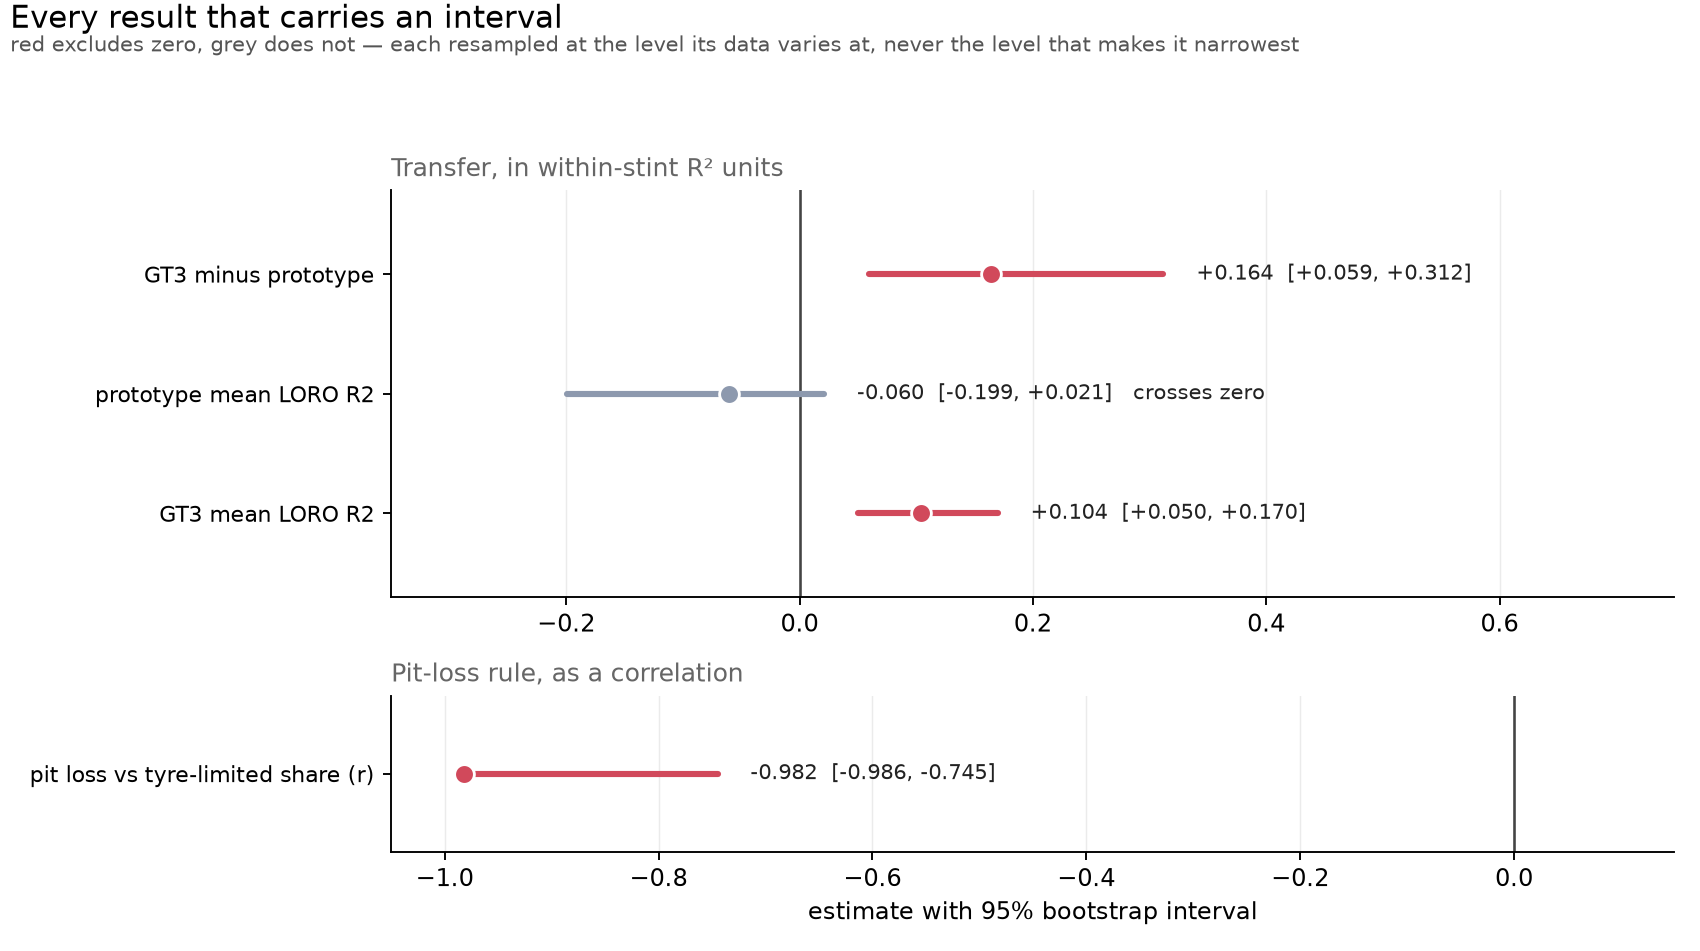
\includegraphics[width=0.92\textwidth]{../reports/figures/s6_intervals.png}
\caption{Every result carrying a bootstrap interval. The two panels are
separate because a within-stint $R^2$ difference and a correlation are not
measured on the same scale, and a forest plot works by letting the reader
compare bar lengths. An earlier single-axis version made the correlation's long
bar read as the strongest result when it is a different measurement. The
cheap-stop edge is absent by design: it is a maximum, and a leave-one-out
sensitivity is reported for it instead of an interval it cannot support.}
\label{fig:intervals}
\end{figure}

The audit's central finding carries no interval, and that is deliberate rather
than an omission. It is a median over decisions that are not independent:
several drivers in one race share a track, a Safety Car and one tyre
allocation. A bootstrap over decisions would understate its width, in the
direction that flatters the result, and a bootstrap over races needs a
clustering the audit table does not carry. Saying so is more useful than
publishing an interval known to be too narrow.

\section{Result 3: an exact optimiser stops later than teams do}

\begin{figure}[htbp]
\centering
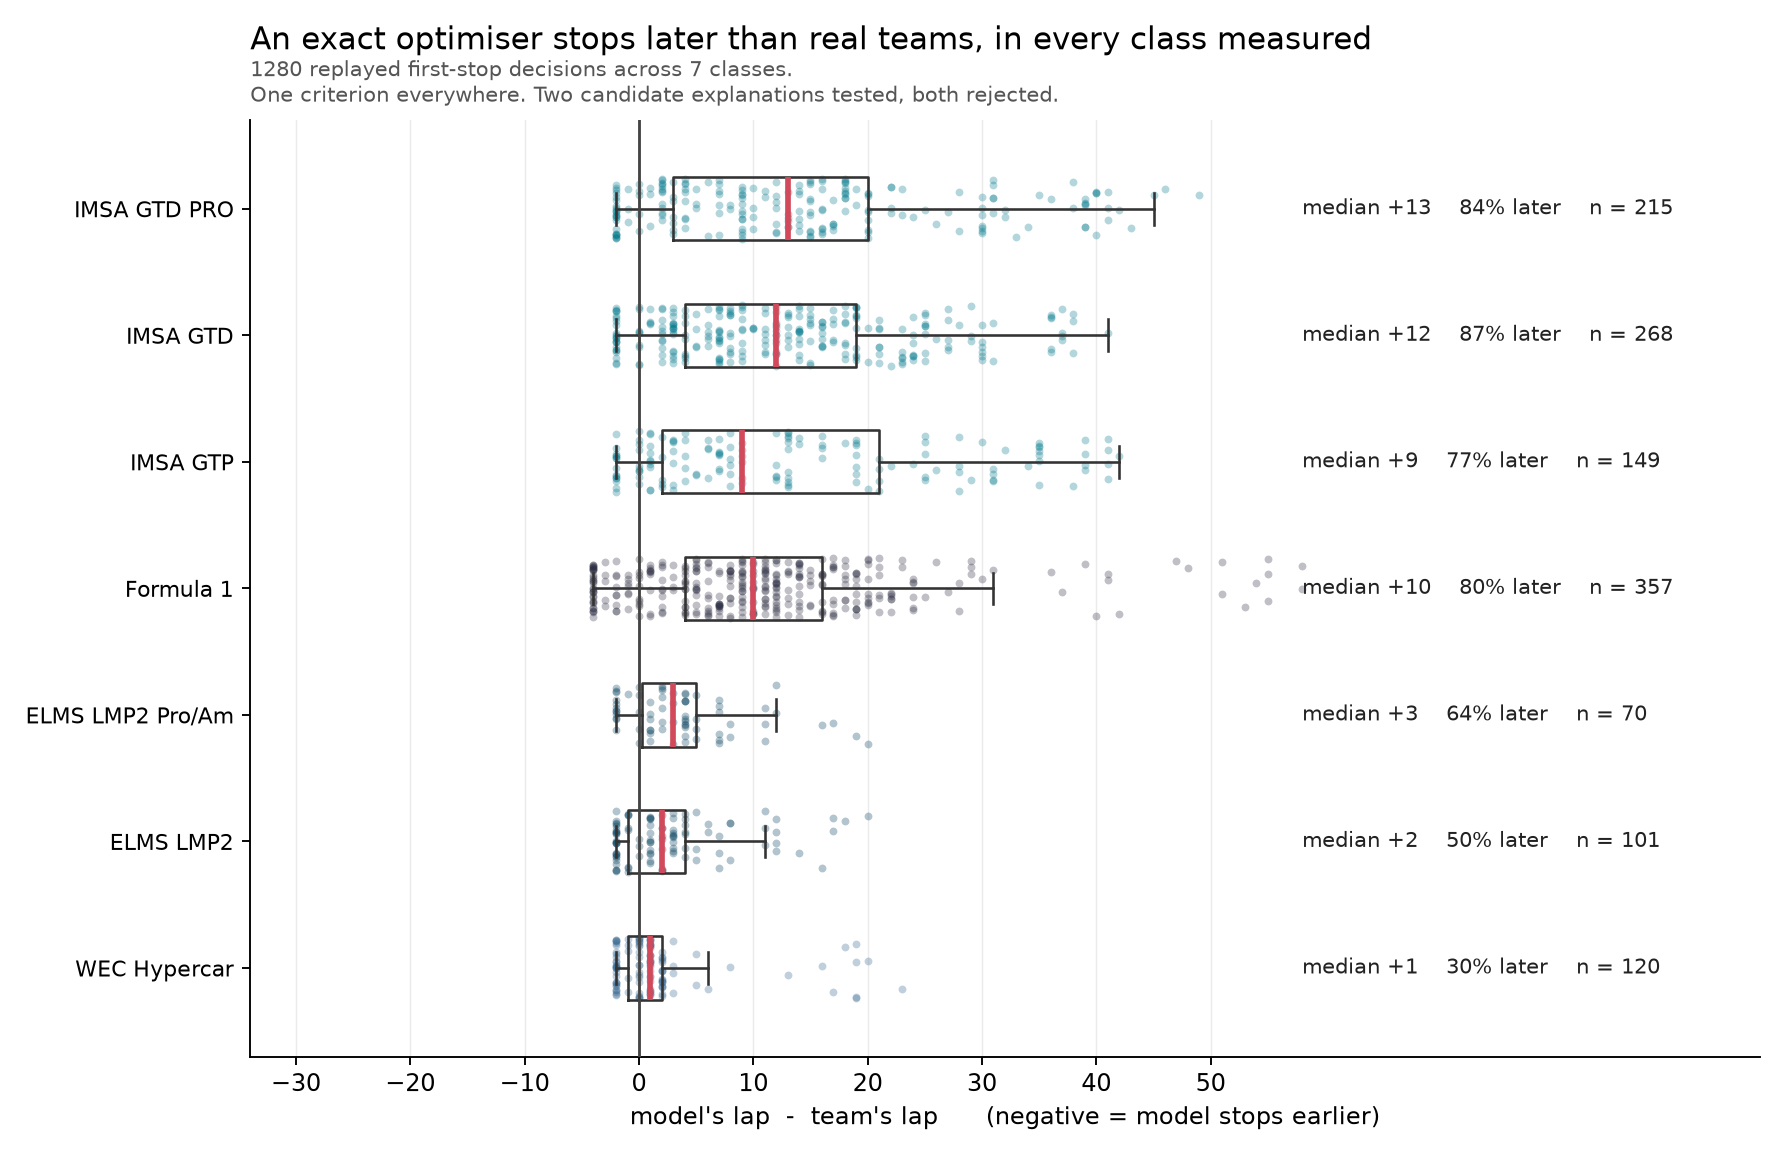
\includegraphics[width=\textwidth]{../reports/figures/r3_audit_bias.png}
\caption{Model lap minus team lap, \NDecisions{} replayed first stops. Box shows
quartiles; the cloud behind it is the sample.}
\label{fig:audit}
\end{figure}

Figure~\ref{fig:audit} shows the whole distribution. Every real first stop
with a fitted model is replayed. The model is asked five
laps before the stop, given the state as it was, and its recommended lap
compared to the team's. This is a replay, not a forecast: the decision point is
defined relative to a stop that already happened, which is what makes the
comparison possible and also what stops it being a prediction claim.

In Formula~1 the optimiser stops later on \FoneLateShare{}\% of decisions, by a
median of \FoneLateMedian{} laps on those; over every decision, late or not, the
median is \FoneMedian{} laps. The endurance figures below are medians over every
decision, so \FoneMedian{} is the comparable one. In endurance the gap tracks the caution rate:
WEC \WecMedian{} laps at \WecCautionShare{}\% of first stops taken under
caution, ELMS \ElmsMedian{} at \ElmsCautionShare{}\%, IMSA \ImsaMedian{} at
\ImsaCautionShare{}\%.

\begin{figure}[htbp]
\centering
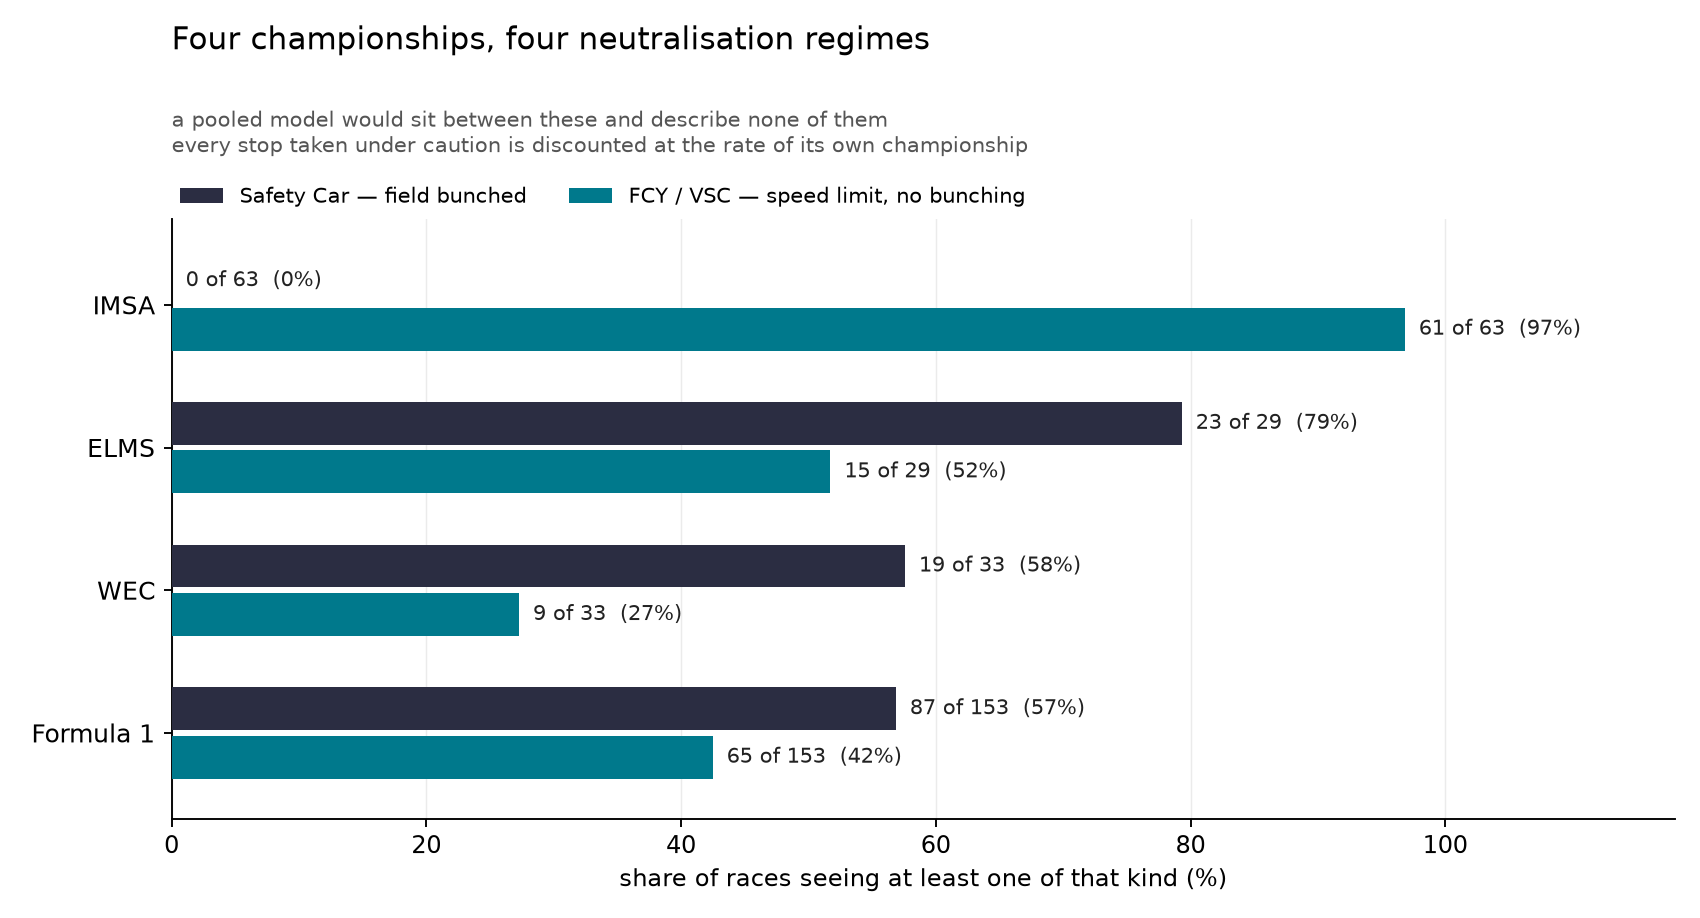
\includegraphics[width=0.9\textwidth]{../reports/figures/s1_neutralisation_regimes.png}
\caption{How often each championship neutralises a race, split by kind. A
Safety Car bunches the field; a Full Course Yellow --- a Virtual Safety Car in
Formula~1 --- imposes a field-wide speed limit without bunching it, and the two
discount the cost of a stop by very different amounts. IMSA deployed no Safety
Car in any scoped race and neutralises almost every race by the other route, so
a figure showing only the first column would put IMSA at zero and contradict
its caution share above. The unit is the race, not the car: the flag is the
modal per-lap flag across the field, never one car's timing row. Classes are
not separated because every class in a race shares the same neutralisation.}
\label{fig:neutralisation}
\end{figure}

Figure~\ref{fig:neutralisation} gives the neutralisation rates behind that
ladder. A stop taken under caution costs a fraction of a green-flag stop, so a
championship that neutralises often gives teams a reason to stop early that the
optimiser, which prices the stop at its green-flag cost, does not see. That
ordering is consistent with the gap, and it is not a test of it: three
championships is three points, and we do not fit a line through them.

\subsection{Testing the two candidate explanations}

We proposed two mechanisms and then attacked them.

\textbf{Absence of track position.} The engine optimises one car's expected race
time and cannot pay for an undercut, which is exactly why a team stops before it
has to. Re-running all \NDecisionsFone{} Formula~1 decisions through a
cover-aware Stackelberg engine consuming each circuit's measured overtaking
difficulty moves the recommendation \emph{away} from the real stop, not toward
it. \textbf{Rejected.}

Across the calendar the cover-aware recommendation lands a median of
\UndercutClosedMedian{} lap further from the real stop than the single-car one,
and only \UndercutShareImproving{}\% of decisions improve at all. Two things
are worth saying about that before it is read as a clean refutation.

The first is that the covariate is thinner than its headline suggests.
Figure~\ref{fig:trackposition} shows a \TrackPositionRange{}-fold range across
\NCircuitsSwap{} circuits, which sounds decisive and is carried by its two
ends. \SwapLowestCircuit{} sits at \SwapLowest{} swaps per lap, a factor of
\SwapRunnerUpRatio{} below the next circuit, with a spread across its
\SwapLowestRaces{} races of only \SwapLowestSd{} --- the one entry that is
genuinely separated. The top of the range rests on \SwapHighestRaces{} races at
a circuit first run in 2023 and is the noisiest row in the table. In between,
the standard deviation across circuits (\SwapBetweenSd{}) is about the same as
the median standard deviation across races within a circuit
(\SwapWithinSd{}), so the twenty circuits in the middle are not separable from
one another on this measure.

The second is that the mechanism is not uniformly wrong. At
\SwapLowestCircuit{}, where overtaking is hardest and the covariate resolves
cleanly, the cover-aware engine does move toward the real stop, by a median of
\SwapLowestClosedMedian{} laps over \SwapLowestDecisions{} decisions, and the
rank correlation between swap rate and improvement is \UndercutSpearman{}
across the calendar. Both point the way the mechanism predicts. Neither is
remotely large enough: half a lap against a median discrepancy of
\FoneMedian{} laps is the right sign at the wrong order of magnitude.
Track position is doing something. It is not doing this.

\begin{figure}[htbp]
\centering
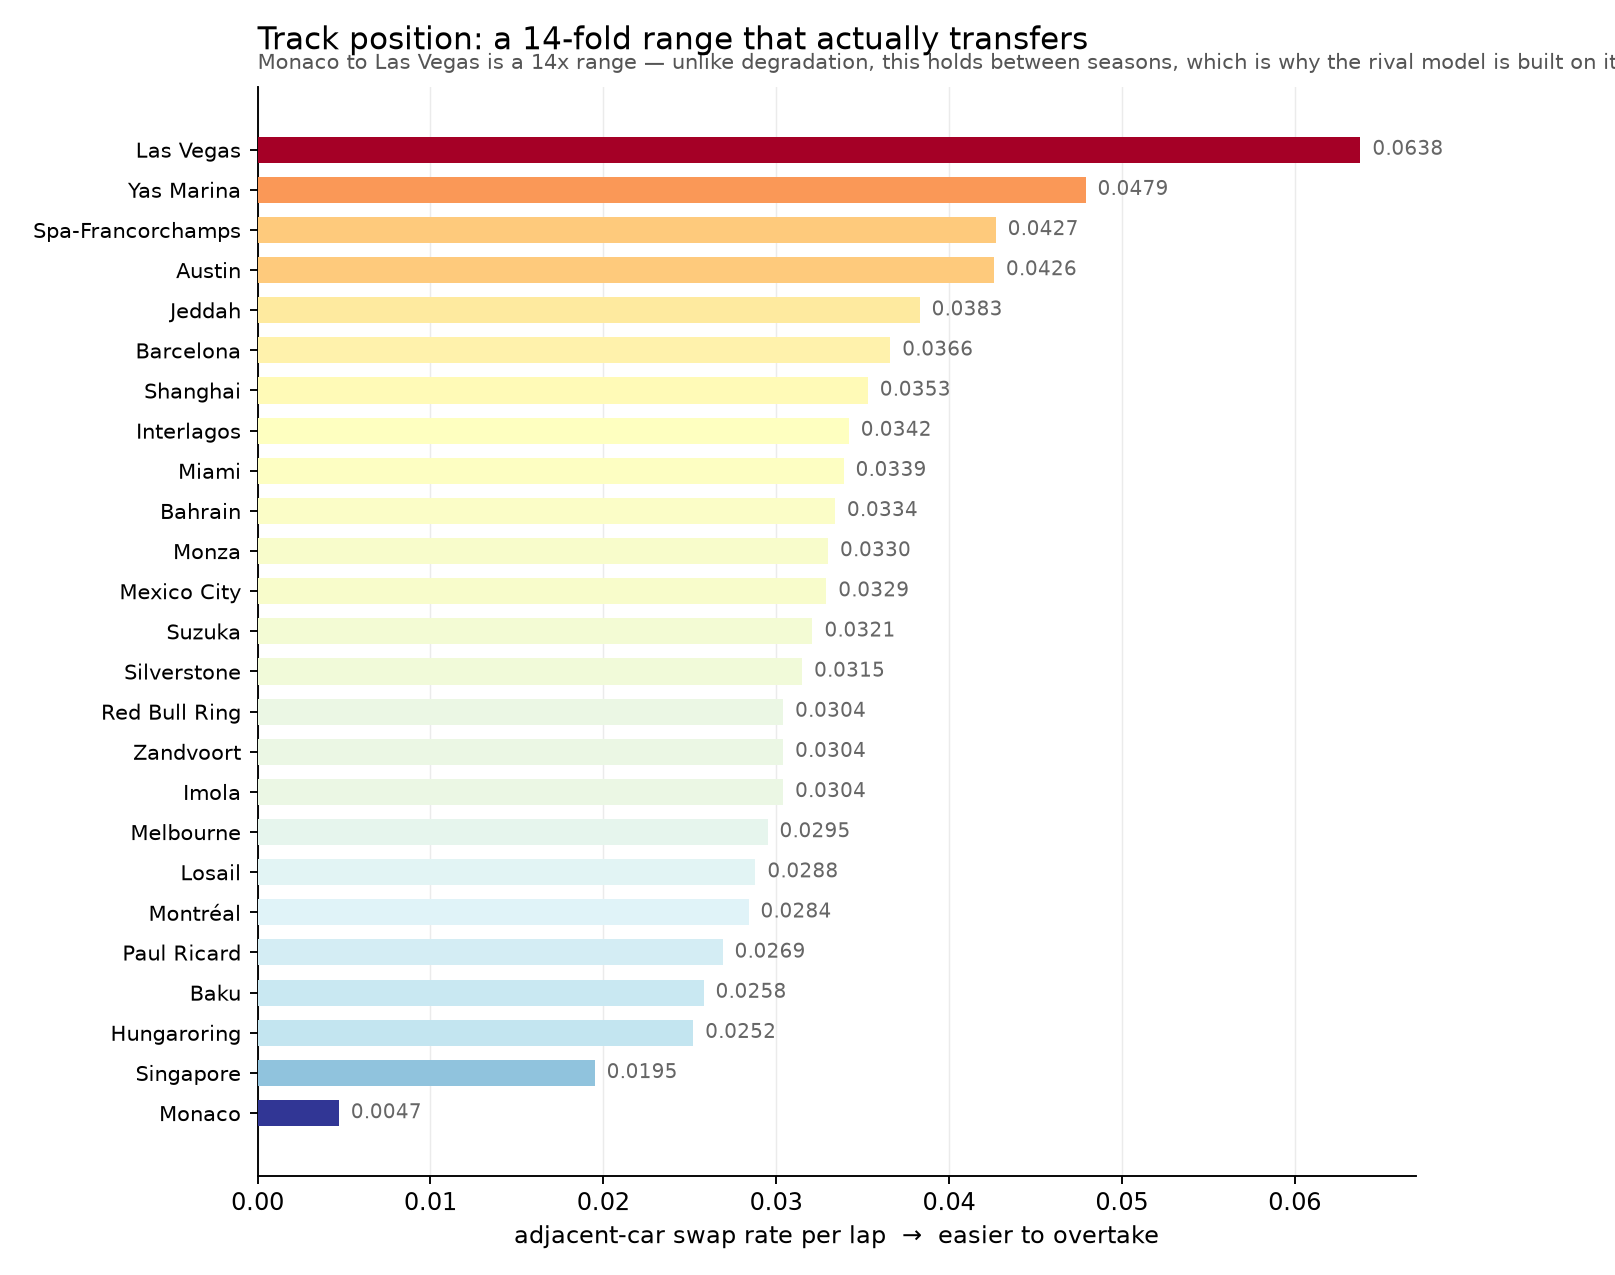
\includegraphics[width=0.78\textwidth]{../reports/figures/s4_track_position.png}
\caption{Adjacent-car swap rate per lap, by circuit. This is the primitive the
cover-aware engine consumes, shown so that the rejection above can be read
against the spread of the input, and not assumed to come from a flat one.}
\label{fig:trackposition}
\end{figure}

\textbf{Slopes biased toward durability.} A tyre that looks flatter than it is
makes staying out look cheaper. Measured against an independent source that
separates tyre wear from fuel burn by a different method on different data, the
median paired difference is negligible --- an error of that size moves a stop by
several race distances, not by ten laps. \textbf{Not detected.} We note that
comparing the two \emph{medians} instead of the median of paired differences
produces a small apparent bias that is an artefact of comparing summaries rather
than pairs; an earlier version of this work nearly reported it.

\subsection{Comparison against three baselines}

\begin{figure}[htbp]
\centering
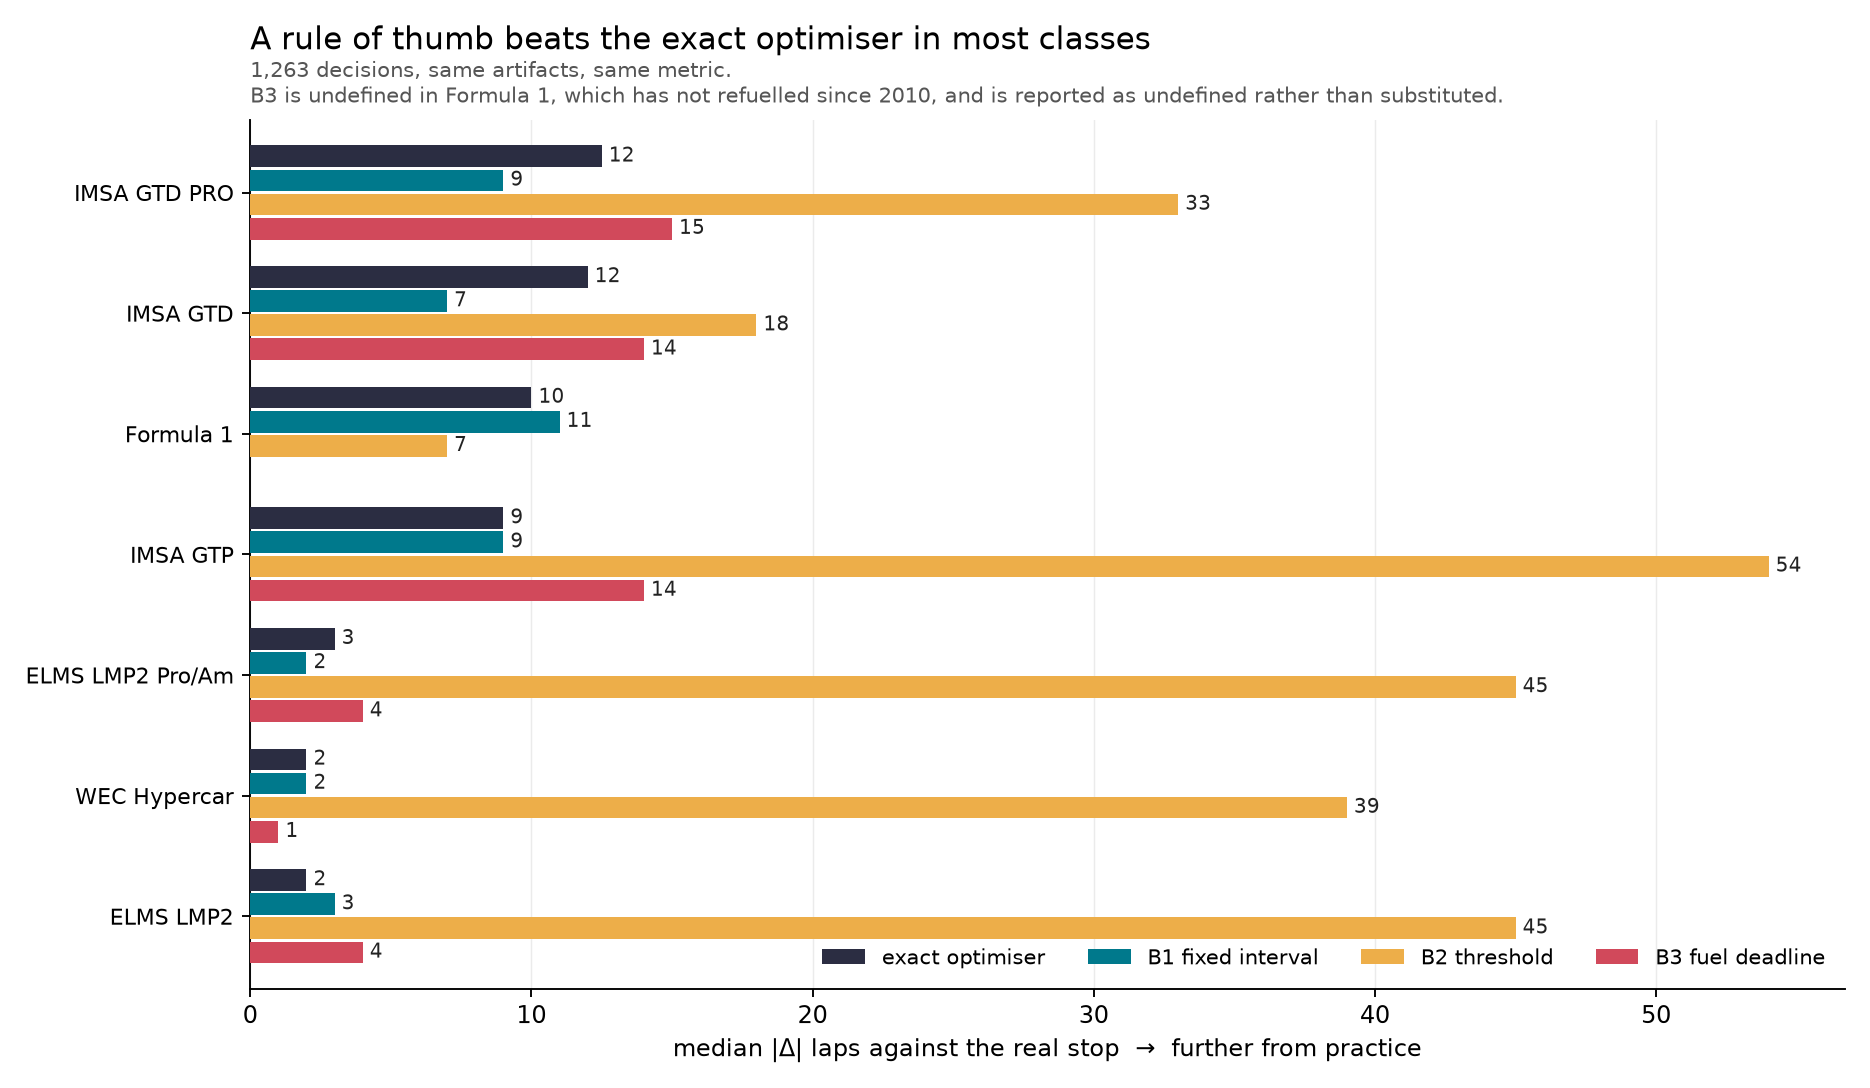
\includegraphics[width=0.92\textwidth]{../reports/figures/s5_baselines.png}
\caption{Median absolute lap error against the real stop, one row per
class rather than per championship. IMSA's three classes run the same rounds
under pit losses of \ImsaGtpPitLoss{}, \ImsaGtdPitLoss{} and
\ImsaGtdproPitLoss{} seconds, so B3 --- run the tank out --- means a different
thing in each and one IMSA row would describe none of them.}
\label{fig:baselines}
\end{figure}

Three rules were scored on \NScored{} of the same decisions, from the same
artifacts, on the same metric (Figure~\ref{fig:baselines} and
Table~\ref{tab:baselines}). B1 divides the race
into equal stints and uses no fitted quantity at all. B2 stops once the tyre's
accumulated loss exceeds the pit loss, using the fitted slope and the measured
pit loss and nothing else. B3 runs the fuel load out, and is undefined in
Formula~1, where refuelling has been prohibited since 2010 --- we report it as
undefined rather than substituting the race end.

Results are reported per class rather than per championship. IMSA runs GTP, GTD
and GTD PRO at the same rounds with median pit losses of \ImsaGtpPitLoss{}, \ImsaGtdPitLoss{} and \ImsaGtdproPitLoss{} seconds,
so a single IMSA row averages three strategy regimes into a number describing
none of them. That grouping also concealed a difference worth seeing: GTP, the
IMSA class with the dearest stops, has the smallest disagreement of the three.

\begin{table}[htbp]
\centering
\caption{Median absolute lap error against the real stop, per class. Lower is
closer to what teams did. B3 is undefined in Formula~1, which has not refuelled
since 2010.}
\label{tab:baselines}
\begin{tabular}{lrrrr}
\toprule
& Optimiser & B1 interval & B2 threshold & B3 fuel \\
\midrule
Formula~1        & \FoneModelError{}            & \FoneBoneError{}            & \textbf{\FoneBtwoError{}}   & \FoneBthreeError{} \\
IMSA GTP         & \ImsaGtpModelError{}         & \ImsaGtpBoneError{}         & \ImsaGtpBtwoError{}         & \ImsaGtpBthreeError{} \\
IMSA GTD         & \ImsaGtdModelError{}         & \textbf{\ImsaGtdBoneError{}}     & \ImsaGtdBtwoError{}    & \ImsaGtdBthreeError{} \\
IMSA GTD PRO     & \ImsaGtdproModelError{}      & \textbf{\ImsaGtdproBoneError{}}  & \ImsaGtdproBtwoError{} & \ImsaGtdproBthreeError{} \\
WEC Hypercar     & \WecHypercarModelError{}     & \WecHypercarBoneError{}     & \WecHypercarBtwoError{}     & \textbf{\WecHypercarBthreeError{}} \\
ELMS LMP2        & \textbf{\ElmsLmptwoModelError{}} & \ElmsLmptwoBoneError{}  & \ElmsLmptwoBtwoError{}      & \ElmsLmptwoBthreeError{} \\
ELMS LMP2 Pro/Am & \ElmsLmptwoProAmModelError{} & \textbf{\ElmsLmptwoProAmBoneError{}} & \ElmsLmptwoProAmBtwoError{} & \ElmsLmptwoProAmBthreeError{} \\
\bottomrule
\end{tabular}
\end{table}

A rule of thumb sits closer to practice than the exact optimiser in
\NClassesRuleWins{} of \NClassesScored{} classes, ties it in
\NClassesRuleTies{} and loses in \NClassesOptimiserWins{}. In
\NClassesBoneWins{} of those classes the winning rule is B1, which uses no
fitted quantity whatsoever --- only the race length and the number of stops
the tank forces. In the two it does not win, it ties the optimiser rather
than losing to it.

Two things this does not establish. \emph{Closer to what teams did} is not
\emph{better}: every number here scores agreement with practice, never which
plan was faster. And it does not rescue the finding --- it removes one more
explanation for it, since the gap cannot come from the simpler methods lacking
information the optimiser has. They have less, and land nearer.

\section{Threats to validity}
\label{sec:threats}

\paragraph{Two withdrawn estimators.} A piecewise race-time basis intended to
absorb track evolution was validated on synthetic races and then withdrawn twice
on real ones: real fields sit close to the degenerate boundary where tyre age
and race time share most of their variance after fixed effects. Formula~1's
median identifiability is \NIdentifiability{}, well outside the range the basis
was shown to work in. We report the omitted variable as diagnosed and unfixed
rather than applying a correction that fails silently.

\paragraph{The audit may not be a fair comparison, and this is the open
question.} The model is asked five laps early and offered every remaining lap,
optimising one car's expected race time. A pit wall is choosing among a handful
of laps inside a strategy already committed to, under a tyre allocation and a
two-compound rule the engine does not represent. We cannot rule out that the
disagreement is an artefact of asking a question no team is answering. Testing
that means constraining the candidate set to what was actually available, which
changes the audit rather than the model.

\paragraph{A fifth of the fitted slopes are not resolved.} Of the
\NCoefficientsFone{} Formula~1 degradation coefficients,
\NCoefCrossingZero{} have a cluster-robust interval containing zero, and
\PctCompoundOverlap{}\% of compound pairs within a circuit have intervals that
overlap each other. Every one of them is carried forward regardless. Screening
on the resolved ones would select on the dependent variable --- circuit-classes
with tight slopes are exactly the ones likeliest to transfer --- and the
transfer result would then be partly an artefact of the screen. The cost is
that the weak transfer reported in Section~\ref{sec:transfer} is a mixture of
genuine instability and of parameters the data never pinned down, and this work
does not separate the two.

\paragraph{Three constants rest on very little.} The cheap-stop edge of
\CheapStopEdge{}\,s is a maximum set by one race; drop it and the edge falls to
\EdgeWithoutDefining{}\,s, \EdgeDropPct{}\%. The second-best transfer score,
\ThinTransfer{} at \ThinTransferWhere{}, is a mean over \ThinTransferFolds{}
folds running from \ThinTransferLow{} to \ThinTransferHigh{} --- a spread of
\ThinTransferSpread{}, wider than most circuit-classes' entire score, and it
should not be read beside \BestTransferWhere{}'s \BestTransfer{}, which
averages \BestTransferFolds{} folds spanning \BestTransferSpread{}. Same
circuit, same protocol, an order of magnitude more stable --- which is itself
worth knowing, since it says the instability is not a property of the circuit
alone. And the top of
the track-position range rests on \SwapHighestRaces{} races at a circuit first
run in 2023. The rules these support are not thin --- \NAboveEdge{}
race-seasons sit above the edge with \NTyreLimitedAboveEdge{} tyre-limited
among them --- but the constants are, and they are quoted here as orders of
magnitude. A full accounting is generated into
\texttt{reports/cross\_series/thin\_evidence.md}.

\paragraph{Compound is unavailable in endurance.} The endurance degradation
models are net-slope models. Comparisons between the Formula~1 per-compound
coefficients and endurance net slopes are made only where the quantity is
genuinely comparable.

\paragraph{Neutralisation regimes are not poolable.} IMSA records no Safety Car
in any scoped race and a Full Course Yellow in nearly all of them; WEC and ELMS
are Safety-Car championships at very different rates. Any pooled endurance
neutralisation model would sit between these and describe none of them, so they
are never merged.

\paragraph{Three layers cannot be regenerated from the repository.} The
breadth-degradation and reliability layers read a third-party export that is not
redistributed here. Their outputs are committed, so every downstream consumer
and every test runs offline; what is blocked is rebuilding them from source.

\section{Reproducibility}

Every artifact derived from committed data is regenerated by continuous
integration, which fails on any difference between the working tree and the
repository --- including files a generator wrote that were never committed, a
blind spot that produced three weeks of silent drift before it was closed.

The state these results were computed from is archived on Zenodo and,
through it, in Software Heritage and OpenAIRE. The concept identifier
\url{https://doi.org/10.5281/zenodo.22726130}
resolves to the newest version of the deposit. The release archived alongside
this paper carries its own frozen identifier, recorded in the repository's
\texttt{CITATION.cff}, for anyone who needs the exact state a figure came from
rather than the current one.

Every number in this manuscript is a macro generated by
\texttt{scripts/make\_paper\_numbers.py} from the committed artifacts; the
source of this paper contains no digits. A separate test recomputes each
published headline from its artifact and asserts the formatted result appears in
the document that publishes it, which is stricter than recomputing alone.

\section{Conclusion}

Degradation slopes rarely transfer, and where they do it is a property of the
circuit-class rather than of the championship or the machinery. Whether an extra
stop can ever pay is decided by the cost of the stop. And an exact optimiser
disagrees with professional practice in a consistent direction that we have not
been able to explain --- having proposed two explanations, tested both, and lost
both, and having found that simpler rules using strictly less information land
closer to what teams actually did in \NClassesRuleWins{} of
\NClassesScored{} classes.

We regard the last of these as the most useful thing here, precisely because it
is unresolved.

\bibliographystyle{plainnat}
\begin{thebibliography}{99}

% Every entry below was checked against a publication record -- Crossref for the
% journal articles, the arXiv API for the preprints -- rather than recalled from
% memory. Two candidate references carried in earlier notes could not be
% confirmed and are deliberately absent. See reports/cross_series/related_work.md.

\bibitem[Aguad and Thraves(2024)]{aguad2024}
Felipe Aguad and Charles Thraves.
\newblock Optimizing pit stop strategies in Formula 1 with dynamic programming
  and game theory.
\newblock \emph{European Journal of Operational Research}, 319(3):908--919,
  2024.
\newblock \doi{10.1016/j.ejor.2024.07.011}.

\bibitem[Bekker and Lotz(2009)]{bekker2009}
James Bekker and Wynand Lotz.
\newblock Planning Formula One race strategies using discrete-event simulation.
\newblock \emph{Journal of the Operational Research Society}, 60(7):952--961,
  2009.
\newblock \doi{10.1057/palgrave.jors.2602626}.

\bibitem[Cameron and Miller(2015)]{cameron2015}
A.~Colin Cameron and Douglas~L. Miller.
\newblock A practitioner's guide to cluster-robust inference.
\newblock \emph{Journal of Human Resources}, 50(2):317--372, 2015.

\bibitem[Cappello and Hoegh(2025)]{cappello2025}
Cole Cappello and Andrew Hoegh.
\newblock A state-space approach to modeling tire degradation in Formula 1
  racing.
\newblock \emph{arXiv preprint arXiv:2512.00640}, 2025.

\bibitem[Carrasco Heine and Thraves(2022)]{carrasco2022}
Oscar~F. Carrasco Heine and Charles Thraves.
\newblock On the optimization of pit stop strategies via dynamic programming.
\newblock \emph{Central European Journal of Operations Research},
  31(1):239--268, 2022.
\newblock \doi{10.1007/s10100-022-00806-4}.

\bibitem[Fieni et~al.(2025)]{fieni2025}
Giona Fieni, Joschua W\"uthrich, Marc-Philippe Neumann, Mohammad~M. Moradi, and
  Christopher~H. Onder.
\newblock Towards learning-based Formula 1 race strategies.
\newblock \emph{arXiv preprint arXiv:2512.21570}, 2025.

\bibitem[Heilmeier et~al.(2018)]{heilmeier2018}
Alexander Heilmeier, Michael Graf, and Markus Lienkamp.
\newblock A race simulation for strategy decisions in circuit motorsports.
\newblock In \emph{2018 21st International Conference on Intelligent
  Transportation Systems (ITSC)}, pages 2986--2993, 2018.
\newblock \doi{10.1109/ITSC.2018.8570012}.

\bibitem[Heilmeier et~al.(2020a)]{heilmeier2020mc}
Alexander Heilmeier, Michael Graf, Johannes Betz, and Markus Lienkamp.
\newblock Application of Monte Carlo methods to consider probabilistic effects
  in a race simulation for circuit motorsport.
\newblock \emph{Applied Sciences}, 10(12):4229, 2020.
\newblock \doi{10.3390/app10124229}.

\bibitem[Heilmeier et~al.(2020b)]{heilmeier2020nn}
Alexander Heilmeier, Andr\'e Thomaser, Michael Graf, and Johannes Betz.
\newblock Virtual strategy engineer: using artificial neural networks for making
  race strategy decisions in circuit motorsport.
\newblock \emph{Applied Sciences}, 10(21):7805, 2020.
\newblock \doi{10.3390/app10217805}.

\bibitem[Santillana(2026)]{santillana2026}
Juan~S. Santillana.
\newblock Pitwall: faithful natural-language race-strategy briefings from a
  calibrated real-time Monte Carlo engine.
\newblock \emph{arXiv preprint arXiv:2607.06495}, 2026.

\bibitem[Thomas et~al.(2025)]{thomas2025}
Devin Thomas, Junqi Jiang, Avinash Kori, Aaron Russo, Steffen Winkler, Stuart
  Sale, Joseph McMillan, Francesco Belardinelli, and Antonio Rago.
\newblock Explainable reinforcement learning for Formula One race strategy.
\newblock \emph{arXiv preprint arXiv:2501.04068}, 2025.

\bibitem[Todd et~al.(2025)]{todd2025}
Jamie Todd, Junqi Jiang, Aaron Russo, Steffen Winkler, Stuart Sale, Joseph
  McMillan, and Antonio Rago.
\newblock Explainable time series prediction of tyre energy in Formula One race
  strategy.
\newblock \emph{arXiv preprint arXiv:2501.04067}, 2025.

\bibitem[van Kampen et~al.(2022)]{vankampen2022}
Jorn van Kampen, Thomas Herrmann, and Mauro Salazar.
\newblock Maximum-distance race strategies for a fully electric endurance race
  car.
\newblock \emph{European Journal of Control}, 68:100679, 2022.
\newblock \doi{10.1016/j.ejcon.2022.100679}.

\end{thebibliography}

\end{document}
